\documentclass[10pt, conference]{IEEEtran}
\usepackage{geometry}
\geometry{a4paper, margin=1in}
\usepackage{graphicx}
\usepackage{amsmath}
\usepackage{enumitem}
\usepackage{paracol}
\usepackage{xcolor}
\usepackage{tabularray}
\usepackage{hyperref}
\usepackage{subcaption}

\title{
Image Generation Using Generative AI with Minimal Objects}

\author{
	\IEEEauthorblockN{Muhammad Hamza}
	\IEEEauthorblockA{
		407251 \\
		Department of Computing \\
		NUST SEECS \\
		\texttt{mhamza.bscs22seecs}\\
		\texttt{@seecs.edu.pk}
}
\and
    \IEEEauthorblockN{Aqsa Batool}
    \IEEEauthorblockA{
	    413777 \\
	    Department of Computing \\
	    NUST SEECS \\
	    \texttt{abatool.bscs22seecs}\\
        \texttt{@seecs.edu.pk}
}
\and
    \IEEEauthorblockN{Ahmed Mohiuddin Shah}
    \IEEEauthorblockA{
        415216 \\
        Department of Computing \\
        NUST SEECS \\
        \texttt{ashah.bscs22seecs}\\
        \texttt{@seecs.edu.pk}
}
}
\begin{document}
\maketitle
\vspace{-1cm}

\section*{Abstract}
Generative AI has advanced image synthesis, but the challenge of creating high-fidelity images using minimal objects remains unresolved. This project introduces a genetic algorithm-based approach to generate images with minimal objects while maintaining image fidelity. The methodology involves initializing a population of objects, applying fitness evaluations using the Delta E color difference metric, and iteratively optimizing through crossover and mutation. Initial prototypes demonstrate the feasibility of achieving high-quality image replication with fewer resources. The proposed method balances computational efficiency and image accuracy, presenting a scalable solution for resource-constrained environments. Future work will refine the model, optimize parameters, and conduct extensive evaluations against existing methods. The project aims to bridge the gap in generative AI by developing a novel, efficient approach to image generation with minimal resource usage.

\section{Introduction}
The rapid advancement of Generative AI has paved the way for innovative applications in various fields, including game design and image synthesis. This project focuses on generating images using a minimal set of objects. The aim is to replicate the original image as accurately as possible while optimizing the number of objects used.

\subsection{Background}
Generative AI has seen significant advancements in recent years, with models like GANs and VAEs capable of generating high-quality images. However, these models often rely on a large number of objects to recreate detailed images. Our project aims to explore methods that can generate images with high fidelity using a minimal set of objects, thereby optimizing computational efficiency and resource utilization.
\subsection{Problem Statement}
The challenge of generating images with minimal objects while maintaining high fidelity poses a significant problem in the field of generative AI. Existing methods often struggle to balance computational efficiency with image accuracy, leading to suboptimal results. This project seeks to address this issue by developing a genetic algorithm-based approach that can generate images with minimal objects while preserving image quality.
\subsection{Research Objectives}
\begin{itemize}
	\item Develop a genetic algorithm-based approach for generating images with minimal objects.
	\item Optimize the model to balance computational efficiency with image fidelity.
	\item Evaluate the performance of the proposed method against existing approaches.
\end{itemize}

\subsection{Problem Identification}
Reconstructing detailed images with a limited set of objects presents a challenge in computer vision and generative algorithms. The main issue is balancing image fidelity with the number of elements used, as current methods often sacrifice computational efficiency for accuracy, or vice versa. This project aims to explore innovative generative models that maintain high image similarity while minimizing object usage.

\subsection{Research Objectives}
The primary objective of this project is to develop a genetic algorithm-based approach for generating images with minimal objects. The model will be optimized to balance computational efficiency with image fidelity, ensuring that the generated images closely resemble the originals. We aim to evaluate the performance of our method against existing approaches to demonstrate its effectiveness in achieving high-quality image generation with minimal resources.

\subsection{Contributions}
\begin{itemize}
	\item Development of a genetic algorithm-based approach for image generation with minimal objects.
	\item Optimization of the model architecture to balance computational efficiency and image fidelity.
	\item Comprehensive evaluation of the proposed method against existing approaches.
	\item Identification of key challenges and opportunities in generative AI for image synthesis.
\end{itemize}

\subsection{Paper Organization}
The paper is organized as follows:
\begin{itemize}
	\item \textbf{Literature Review:} Discusses the background and evolution of genetic algorithms in image processing.
	\item \textbf{Research Gap Identification:} Identifies the research gap and motivates the need for our proposed approach.
	\item \textbf{System Design Model:} Outlines the methodology and approach for image generation using genetic algorithms.
	\item \textbf{Project Methodology:} Describes the initial prototypes and testing conducted to validate the proposed approach.
	\item \textbf{Implementation and Results:} Presents the results of the initial tests and outlines the next steps in the project.
	\item \textbf{Disccusion and Conclusion:} Discusses the implications of the research findings and outlines future work.
	\item \textbf{Conclusion and Future Work:} Summarizes the key findings and contributions of the research and suggests avenues for future work.
	\item \textbf{References:} Lists the references cited in the paper.
	\item \textbf{Appendix:} Includes additional information, such as code snippets or detailed experimental results.
\end{itemize}


\section{Literature Review}
Genetic algorithms (GAs) have long been celebrated for their ability to mimic evolutionary processes and adapt complex problem-solving approaches inspired by natural selection. Originating from the work of John Holland, these algorithms are rooted in mechanisms akin to biological evolution, specifically natural selection and genetic recombination \hypertarget{ref}{\textsuperscript{\hyperref[sec:1r]{[1]}\label{sec:1}}}. GAs simulate the "survival of the fittest" paradigm, where the selection, crossover, and mutation of potential solutions iteratively refine the population towards more optimal solutions \hypertarget{ref}{\textsuperscript{\hyperref[sec:2r]{[2]}\label{sec:2}}}. The foundational concepts, alongside enhancements to these processes, have been applied to diverse domains, including image reconstruction and data analysis \hypertarget{ref}{\textsuperscript{\hyperref[sec:1r]{[1]}\label{sec:1}}}. \\

Holland's early exploration and subsequent popularization of GAs highlighted their capability to overcome the traditional hurdles of algorithmic problem-solving by employing principles of natural selection and genetic diversity \hypertarget{ref}{\textsuperscript{\hyperref[sec:2r]{[2]}\label{sec:2}}}. His methods laid the groundwork for the algorithmic framework that would be expanded upon by later researchers \hypertarget{ref}{\textsuperscript{\hyperref[sec:3r]{[3]}\label{sec:3}}}. For instance, the classical structure of GAs involves initializing a population with potential solutions, assessing their fitness, and applying crossover and mutation operators to generate new populations. This iterative method fosters the development of solutions by combining the best traits of parent individuals \hypertarget{ref}{\textsuperscript{\hyperref[sec:3r]{[3]}\label{sec:3}}}. \\

Recent studies have expanded the application of GAs to image processing and artistic creation. One notable area of investigation is the use of GAs to reconstruct binary or non-photo-realistic images from random initial conditions \hypertarget{ref}{\textsuperscript{\hyperref[sec:1r]{[1]}\label{sec:1}}}\hypertarget{ref}{\textsuperscript{\hyperref[sec:5r]{[5]}\label{sec:5}}}. By using techniques such as crossover and mutation, these algorithms can generate abstract or painterly images that evolve over successive generations, providing insights into both the algorithm's creative potential and its technical limitations \hypertarget{ref}{\textsuperscript{\hyperref[sec:5r]{[5]}\label{sec:5}}}\hypertarget{ref}{\textsuperscript{\hyperref[sec:6r]{[6]}\label{sec:6}}}. This application is particularly relevant as researchers explore how genetic algorithms can go beyond traditional data processing into realms of artistic expression and visualization.\\

Further advancements in multi-objective genetic algorithms (MOGAs) have introduced methods to address complex optimization problems, such as recovering lost image data during compression or resizing \hypertarget{ref}{\textsuperscript{\hyperref[sec:4r]{[4]}\label{sec:4}}}. The scalability of such approaches, especially when implemented in distributed systems, highlights their practical utility in cloud computing and data transmission. These methods demonstrate how GAs can leverage parallel computing power to optimize space without compromising significant image details, thus showcasing their adaptability to real-world data processing needs \hypertarget{ref}{\textsuperscript{\hyperref[sec:4r]{[4]}\label{sec:4}}}.\\

Moreover, the representation of individuals within GAs has evolved over time, impacting their effectiveness in creative and computational tasks. Traditional approaches often utilized simple data structures, but recent experiments have implemented individuals as complex entities, such as arrays of RGB values, allowing for detailed image manipulations \hypertarget{ref}{\textsuperscript{\hyperref[sec:5r]{[5]}\label{sec:5}}}. This diversification in individual representation has opened up novel possibilities for evolutionary art, where genetic algorithms are harnessed to generate unique, aesthetic images that mirror the painterly styles traditionally associated with human artists \hypertarget{ref}{\textsuperscript{\hyperref[sec:6r]{[6]}\label{sec:6}}}. The success of these approaches emphasizes the potential of GAs to merge computation with creativity, demonstrating their broad applicability and versatility in solving a wide array of problems. \\


Genetic Algorithms (GAs) have been applied to various image processing tasks, including AI image generation, steganography, and segmentation. Salvaggio (2023) explored the use of GANs trained on personal photos, revealing distortions in memory and imagination \hypertarget{ref}{\textsuperscript{\hyperref[sec:7r]{[7]}\label{sec:7}}}. Shyla et al. (2021) improved image steganography by optimizing carrier image selection and secret data embedding, achieving up to 40\% better performance \hypertarget{ref}{\textsuperscript{\hyperref[sec:8r]{[8]}\label{sec:8}}}. Jedlicka and Ryba found that GAs provided comparable or superior results to other segmentation methods, though with higher computational demands \hypertarget{ref}{\textsuperscript{\hyperref[sec:9r]{[9]}\label{sec:9}}}. These studies highlight GAs' effectiveness in image optimization tasks. \\

Sit et al. (2022) reviewed the use of GAs for image reconstruction, highlighting potential improvements in key operators like selection, crossover, and mutation to enhance reconstruction speed and image quality \hypertarget{ref}{\textsuperscript{\hyperref[sec:10r]{[10]}\label{sec:10}}}. Fenaux et al. (2023) introduced Gaggle, a PyTorch-based library for evolutionary algorithms (EAs), improving GPU support for neuroevolution tasks and offering significant runtime improvements over previous libraries \hypertarget{ref}{\textsuperscript{\hyperref[sec:11r]{[11]}\label{sec:11}}}. Khan et al. (2021) explored the applications of genetic programming (GP) in image processing, emphasizing its versatility in fields like medical imaging, compression, and pattern recognition, and providing guidelines for future research \hypertarget{ref}{\textsuperscript{\hyperref[sec:12r]{[12]}\label{sec:12}}}. \\

Projects like Triangula leverage GAs to approximate images using triangles and polygons, showcasing the flexibility of GAs in image representation \hypertarget{ref}{\textsuperscript{\hyperref[sec:13r]{[13]}\label{sec:13}}}. Similarly, Spu7Nix's work on generating videos in Geometry Dash through GAs demonstrates their application in creative media generation \hypertarget{ref}{\textsuperscript{\hyperref[sec:14r]{[14]}\label{sec:14}}}. In hyperparameter optimization, GAs outperform traditional methods like Grid Search and Random Search, particularly for neural architecture search (NAS), as shown by Liashchynskyi et al. \hypertarget{ref}{\textsuperscript{\hyperref[sec:15r]{[15]}\label{sec:15}}}. Additionally, GAs have been applied in a variety of optimization tasks, such as modeling and material discovery, with notable efficiency gains when combined with machine learning methods \hypertarget{ref}{\textsuperscript{\hyperref[sec:16r]{[16]}\label{sec:16}}}\hypertarget{ref}{\textsuperscript{\hyperref[sec:17r]{[17]}\label{sec:17}}}. \\

In the domain of medical and pathology image segmentation, improved GAs have demonstrated superior performance. Huang et al. (2024) proposed enhancements to GA for multi-threshold optimization in digital pathology, improving segmentation accuracy and computational efficiency \hypertarget{ref}{\textsuperscript{\hyperref[sec:18r]{[18]}\label{sec:18}}}. Alam et al. (2020) discussed the role of GAs in solving complex optimization problems, particularly in engineering, highlighting their versatility in addressing hybrid computational challenges \hypertarget{ref}{\textsuperscript{\hyperref[sec:19r]{[19]}\label{sec:19}}}. Moreover, advancements in edge detection algorithms, such as the Log Sobel operator, further enhance the precision and speed of image processing tasks \hypertarget{ref}{\textsuperscript{\hyperref[sec:20r]{[20]}\label{sec:20}}}. \\

In summary, genetic algorithms have proven to be robust tools capable of solving highly varied and complex problems by emulating the processes of evolution.
Genetic Algorithms (GAs), inspired by natural evolution, are used for solving complex optimization problems by iterating through selection, crossover, and mutation processes. They have been applied in diverse areas, including image reconstruction, artistic creation, and optimization tasks. GAs enable creative applications such as generating non-photo-realistic images and enhancing image data recovery. Recent advancements include multi-objective GAs (MOGAs) for complex optimization and improvements in representation, like RGB arrays, enhancing their effectiveness in creative and computational tasks. GAs are also used in AI image generation, steganography, and segmentation, showing notable performance in comparison to traditional methods.

\section{Research Gap Identification}
While existing research highlights various generative techniques, few approaches emphasize achieving high-fidelity images using minimal objects. Most current solutions lack efficiency when applied to resource-constrained environments. We aim to introduce an optimized method for image reconstruction that ensures both accuracy and minimal object usage.

\section{System Design Model}
Our proposed system design model leverages genetic algorithms to generate images with minimal objects. The model architecture consists of the following components:
\begin{itemize}
	\item \textbf{Genetic Algorithm:} The core algorithm responsible for evolving the population of objects to generate images.
	\item \textbf{Fitness Function:} Evaluates the similarity between the generated and original images to guide the optimization process.\\
	      \begin{figure}[h!]
		      \centering
		      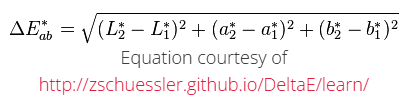
\includegraphics[width=0.5\linewidth]{delta_e.png}
		      \caption{Delta E Formula}
	      \end{figure} \\
	      We used the \textbf{Delta E}\hypertarget{ref}{\textsuperscript{\hyperref[sec:21r]{[21]}\label{sec:21}}} color difference metric to calculate the fitness of the generated image. The Delta E formula measures the perceptual difference between two colors, providing a quantitative measure of color accuracy. By comparing the RGB values of the generated and original images, we can calculate the Delta E value to assess the fitness of the generated image.
	\item \textbf{Crossover and Mutation Operators:} Enable the exploration of the solution space by combining and modifying objects.
	\item \textbf{Population Initialization:} Initializes the population of objects with random values to kickstart the optimization process.
	\item \textbf{Image Representation:} Represents images as a set of objects (e.g., ellipses, polygons) to reconstruct the original image.
\end{itemize}

\section{Project Methodology}

\subsection{Techniques and Algorithms}
Our project primarily utilizes genetic algorithms to generate images with minimal objects. The genetic algorithm iteratively evolves a population of objects to approximate the original image. The fitness function evaluates the similarity between the generated and original images, guiding the optimization process. Crossover and mutation operators enable the exploration of the solution space by combining and modifying objects.

\subsection{Architecture Diagram}
\begin{figure}[h!]
	\centering
	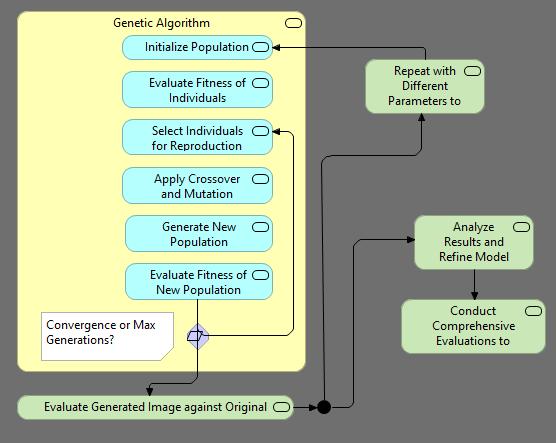
\includegraphics[width=0.8\linewidth]{architecture_diagram.png}
	\caption{System Architecture Diagram}
\end{figure}

\subsection{Process Flow}
\begin{enumerate}
	\item Initialize the population with random objects.
	\item Evaluate the fitness of each individual in the population.
	\item Select individuals for reproduction based on their fitness.
	\item Apply crossover and mutation operators to generate new individuals.
	\item Evaluate the fitness of the new population.
	\item Repeat the process until convergence or a specified number of generations.
	\item Output the best individual as the generated image.
	\item Evaluate the generated image against the original image.
	\item Repeat the process with different parameters to optimize the model.
	\item Analyze the results and refine the model architecture.
	\item Conduct comprehensive evaluations to benchmark performance.
\end{enumerate}

\subsection{Alignment}
The proposed methodology aligns seamlessly with the system design model, leveraging genetic algorithms to generate images with minimal objects. The architecture diagram illustrates the core components of the system, including the genetic algorithm, fitness function, crossover and mutation operators, and population initialization. The process flow outlines the step-by-step execution of the system, from population initialization to result evaluation, ensuring a coherent and structured approach to image generation.

\section{Implementation and Results}

\subsection*{
	Initial Test
}
We did an initial test with 10,000 generation steps on a basic model which only uses ellipses:
\begin{figure}[h!]
	\centering
	\begin{subfigure}{0.4\linewidth}
		\centering
		
\includegraphics[width=\linewidth]{eren orig.png}
		\caption{Original Image}
	\end{subfigure}%
	\hfill
	\begin{subfigure}{0.4\linewidth}
		\centering
		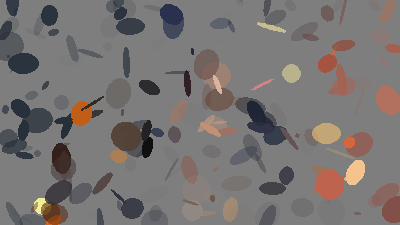
\includegraphics[width=\linewidth]{generated_100.png}
		\caption{100 generations}
	\end{subfigure}
	\begin{subfigure}{0.4\linewidth}
		\centering
		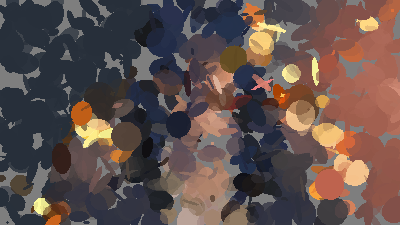
\includegraphics[width=\linewidth]{generated_9900.png}
		\caption{9900 generations}
	\end{subfigure}
	\caption{Recreating original image using basic Algoritm Implementation}
\end{figure}

Using the fitness graph, we can see that our fitness has stagnated and is not improving much further.

\subsection*{
	Difference between original and generated image
}
We calculated the difference between the original and generated image to evaluate the image fidelity. The difference images show the discrepancies between the original and generated images, highlighting areas where the generated image deviates from the original.

\begin{figure}[h!]
	\centering
	\begin{subfigure}{0.4\linewidth}
		\centering
		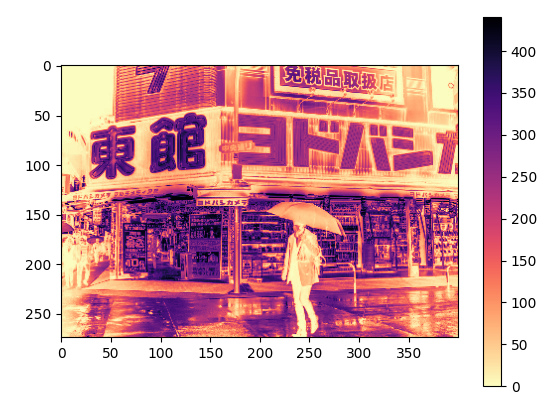
\includegraphics[width=\linewidth]{Screenshot 2025-01-02 172336.png}
		\caption{Difference of Blank Canvas}
	\end{subfigure}
	\begin{subfigure}{0.4\linewidth}
		\centering
		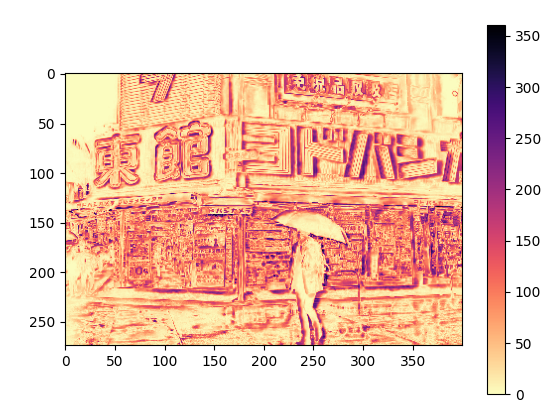
\includegraphics[width=\linewidth]{Screenshot 2025-01-02 172237.png}
		\caption{Difference of cb image}
	\end{subfigure}
	\caption{Difference between original and generated image}
\end{figure}

\subsection*{
	Improved Model
}
We then implemented a more complex model that diminishes the size of the ellipses as the generation progresses. This model showed better results in terms of fitness and image fidelity.

\begin{figure}[h!]
	\centering
	\begin{subfigure}{0.4\linewidth}
		\centering
		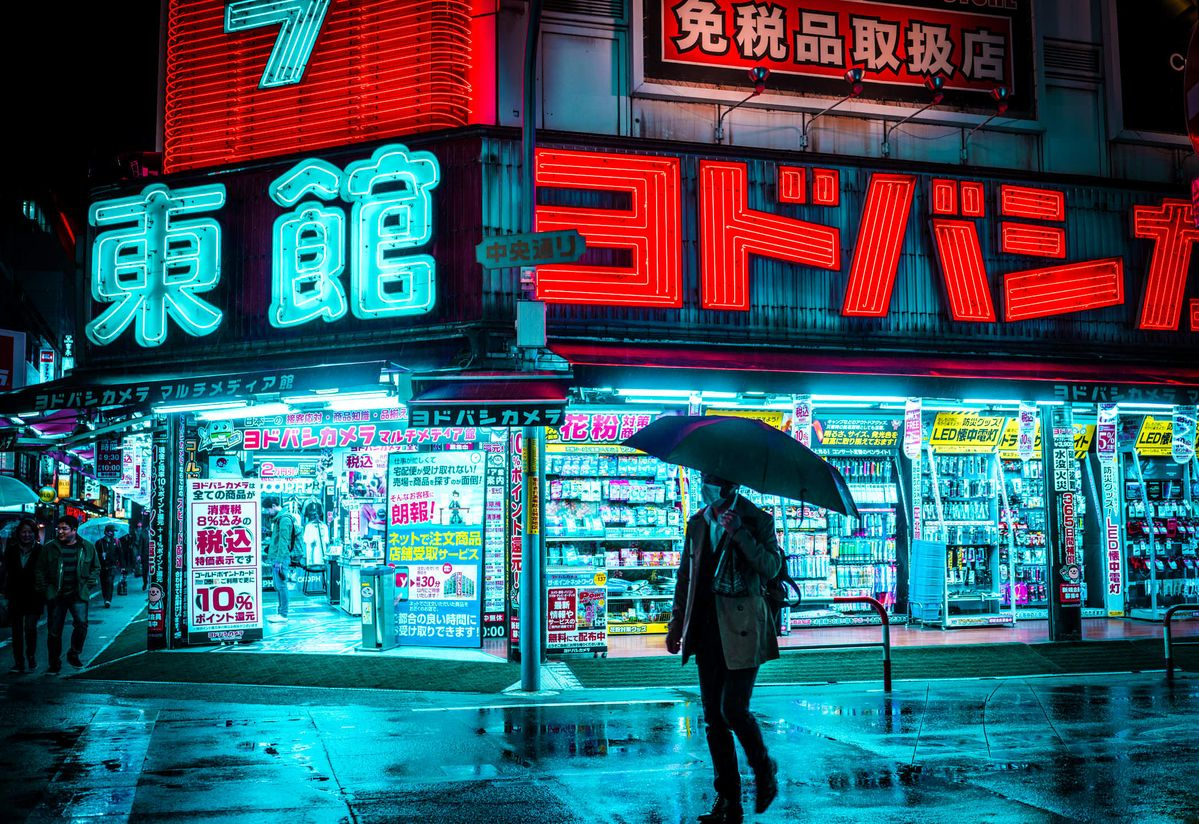
\includegraphics[width=\linewidth]{cbpunk.jpg}
		\caption{Original Image}
	\end{subfigure}%
	\hfill
	\begin{subfigure}{0.4\linewidth}
		\centering
		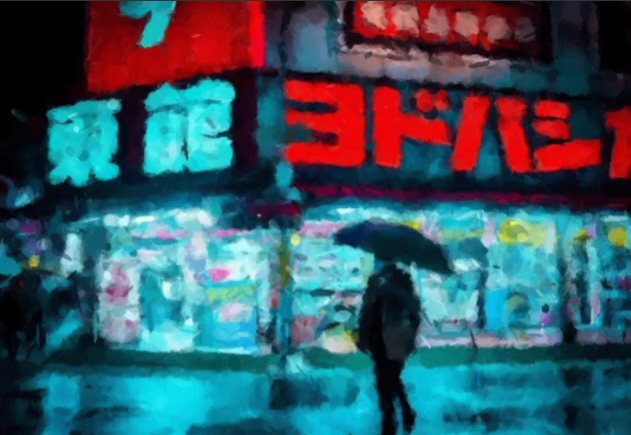
\includegraphics[width=\linewidth]{Screenshot 2025-01-02 172200.png}
		\caption{After 50,000 generations}
	\end{subfigure}
	\begin{subfigure}{0.8\linewidth}
		\centering
		
\includegraphics[width=\linewidth]{Screenshot 2025-01-02 173147.png}
		\caption{50,000 generations for eren image}
	\end{subfigure}
	\begin{subfigure}{0.8\linewidth}
		\centering
		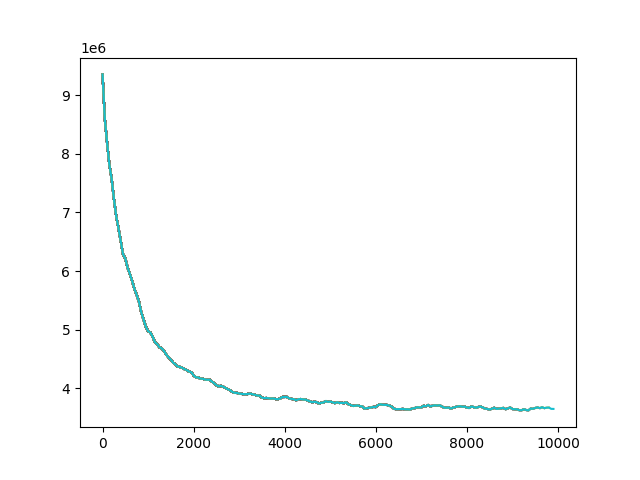
\includegraphics[width=\linewidth]{fitness_generation_9900.png}
		\caption{Fitness Graph}
	\end{subfigure}
	\caption{Recreating original image using improved Algoritm Implementation}
\end{figure}

As shown in the results, the improved model demonstrates better fitness and image fidelity compared to the basic model. The fitness graph indicates a more consistent improvement in fitness over the generations, suggesting that the model is converging towards the original image.\\
We observed that after a certain number of generations, the fitness value stagnates, indicating that the model has reached a local optimum. This highlights the need to optimize the model parameters and explore different representations and fitness functions to enhance convergence and image fidelity.

\subsection*{
	Next Steps
}
\begin{itemize}
	\item Refine the model architecture to improve convergence and image fidelity.
	\item Experiment with different object representations and fitness functions.
	\item Optimize the genetic algorithm parameters to enhance performance.
	\item Conduct comprehensive evaluations to benchmark the model against existing methods.
	\item Analyze the results and refine the model architecture.
	\item Explore parallelization and distributed computing to improve scalability.
\end{itemize}



\section{Contributions of Each Member}

\begin{enumerate}[label=\arabic*)]
	\item \textbf{Aqsa Batool}: Conducted literature review and analyzed existing methods focused on object constraints. Created Fitness Functions.
	\item \textbf{Muhammad Hamza}: Focused on comparing traditional approaches and implementing optimization techniques.
	\item \textbf{Ahmed Mohiuddin Shah}: Led prototype development and testing and analyzed hardware constraints.
\end{enumerate}

\section{Disccusion}
The initial tests have shown promising results, with the improved model demonstrating better fitness and image fidelity. The next steps involve refining the model architecture, experimenting with different object representations and fitness functions, and optimizing the genetic algorithm parameters. The comprehensive evaluations will provide insights into the model's performance and scalability, guiding further refinements and enhancements. The project aims to address the research gap by developing an optimized method for image generation with minimal objects, balancing computational efficiency with image fidelity.

\section{Conclusion and Future Work}
In conclusion, the proposed genetic algorithm-based approach shows potential for generating images with minimal objects while maintaining high fidelity. The initial tests have yielded promising results, and the improved model demonstrates better fitness and image fidelity. The next steps involve refining the model architecture, optimizing the genetic algorithm parameters, and conducting comprehensive evaluations to benchmark the model against existing methods. The project aims to address the research gap by developing an optimized method for image generation with minimal objects, balancing computational efficiency with image fidelity. Future work will focus on enhancing the model's performance, scalability, and applicability to real-world scenarios.

\section{References}
\begin{itemize}
	\item \textbf{\hyperref[sec:1]{[1]}\label{sec:1r}}Mirjalili, S., Song Dong, J., Sadiq, A.S., Faris, H. (2020). Genetic Algorithm: Theory, Literature Review, and Application in Image Reconstruction. In: Mirjalili, S., Song Dong, J., Lewis, A. (eds) Nature-Inspired Optimizers. Studies in Computational Intelligence, vol 811. Springer, Cham.
	      \url{https://doi.org/10.1007/978-3-030-12127-3_5}

	\item \textbf{\hyperref[sec:2]{[2]}\label{sec:2r}}Holland, J. H. (1992). Genetic Algorithms. Scientific American, 267(1), 66–73. \url{http://www.jstor.org/stable/24939139}
	\item \textbf{\hyperref[sec:3]{[3]}\label{sec:3r}}Genetic Algorithms
	      STEPHANIE FORREST
	      Department of Computer Science, University of New Mexico, Albuquerque forrest@cs.unm.edu
	      \url{https://dl.acm.org/doi/pdf/10.1145/234313.234350}
	\item \textbf{\hyperref[sec:4]{[4]}\label{sec:4r}}A Genetic Algorithm Approach to Regenerate Image from a Reduce Scaled Image Using Bit Data Count Kishor Datta Gupta Ph.D. Student, Computer Science University of Memphis, United States of America 3720 Alumni Ave, Memphis, TN 38152, USA kdgupt1@memphis.edu Sajib Sen Ph.D. Student, Computer Science University of Memphis, United States of America 3720 Alumni Ave, Memphis, TN 38152, USA ssen4@memphis.edu \url{https://lumenpublishing.com/journals/index.php/brain/article/view/2031/1688}

	\item \textbf{\hyperref[sec:5]{[5]}\label{sec:5r}}\url{https://github.com/SebastianCharmot/Genetic-Algorithm-Image-Recreation/blob/master/CSC_370_Final_Project_Sebastian_Daniel.pdf}
	      Genetic Programming for Non-Photorealistic Image Generation
	      Sebastian Charmot and Daniel Cowan
	      secharmot,
	      dacowan@
	      davidson.edu
	      Davidson College
	      Davidson, NC 28035
	      U.S.A.

	\item \textbf{\hyperref[sec:6]{[6]}\label{sec:6r}}Baniasadi, M., Ross, B.J. Exploring non-photorealistic rendering with genetic programming. Genet Program Evolvable Mach 16, 211–239 (2015). \url{https://doi.org/10.1007/s10710-014-9234-0}

	\item \textbf{\hyperref[sec:7]{[7]}\label{sec:7r}}	      Eryk Salvaggio; Infinite Barnacle: The AI Image and Imagination in GANs from Personal Snapshots. Leonardo 2023; 56 (6): 575–578. doi: \url{https://doi.org/10.1162/leon_a_02404}

	\item \textbf{\hyperref[sec:8]{[8]}\label{sec:8r}}      M.K. Shyla, K.B. Shiva Kumar, Rajendra Kumar Das,
	      Image steganography using genetic algorithm for cover image selection and embedding,
	      Soft Computing Letters,
	      Volume 3,
	      2021,
	      100021,
	      ISSN 2666-2221,
	      \url{https://doi.org/10.1016/j.socl.2021.100021}
	\item \textbf{\hyperref[sec:9]{[9]}\label{sec:9r}}	      Jedlicka, P., Ryba, T. Genetic algorithm application in image segmentation. Pattern Recognit. Image Anal. 26, 497–501 (2016). \url{https://doi.org/10.1134/S105466181603007X}
	\item \textbf{\hyperref[sec:10]{[10]}\label{sec:10r}}
	      Enhanced Genetic Algorithm in Image Reconstruction \url{https://ieeexplore.ieee.org/document/9952096}
	\item \textbf{\hyperref[sec:11]{[11]}\label{sec:11r}} Lucas Fenaux, Thomas Humphries, and Florian Kerschbaum. 2023. Gaggle: Genetic Algorithms on the GPU using PyTorch. In Proceedings of the Companion Conference on Genetic and Evolutionary Computation (GECCO '23 Companion). Association for Computing Machinery, New York, NY, USA, 2358–2361. \url{https://doi.org/10.1145/3583133.3596356 }
	\item \textbf{\hyperref[sec:12]{[12]}\label{sec:12r}} A recent survey on the applications of genetic programming in image processing
	      Asifullah Khan, Aqsa Saeed Qureshi, Noorul Wahab, Mutawarra Hussain, Muhammad Yousaf Hamza
	      First published: 01 June 2021 \url{https://doi.org/10.1111/coin.12459}
	\item \textbf{\hyperref[sec:13]{[13]}\label{sec:13r}} Grid Search, Random Search, Genetic Algorithm: A Big Comparison for NAS
	      Petro Liashchynskyi, Pavlo Liashchynskyi \url{https://doi.org/10.48550/arXiv.1912.06059}
	\item \textbf{\hyperref[sec:14]{[14]}\label{sec:14r}} John McCall,
	      Genetic algorithms for modelling and optimisation,
	      Journal of Computational and Applied Mathematics,
	      Volume 184, Issue 1,
	      2005,
	      Pages 205-222,
	      ISSN 0377-0427, \url{https://doi.org/10.1016/j.cam.2004.07.034}
	\item \textbf{\hyperref[sec:15]{[15]}\label{sec:15r}}
	      Jennings, P.C., Lysgaard, S., Hummelshøj, J.S. et al. Genetic algorithms for computational materials discovery accelerated by machine learning. npj Comput Mater 5, 46 (2019). \url{https://doi.org/10.1038/s41524-019-0181-4}
	\item \textbf{\hyperref[sec:16]{[16]}\label{sec:16r}}
	      Huang, T., Yin, H. \& Huang, X. Improved genetic algorithm for multi-threshold optimization in digital pathology image segmentation. Sci Rep 14, 22454 (2024). \url{https://doi.org/10.1038/s41598-024-73335-6}
	\item \textbf{\hyperref[sec:17]{[17]}\label{sec:17r}}
	      Genetic Algorithm: Reviews, Implementations, and Applications,  Tanweer Alam, Shamimul Qamar, Amit Dixit, Mohamed Benaida
	      \url{https://doi.org/10.48550/arXiv.2007.12673}
	\item \textbf{\hyperref[sec:18]{[18]}\label{sec:18r}}Guowei Yang, Fengchang Xu,
	      Research and analysis of Image edge detection algorithm Based on the MATLAB,
	      Procedia Engineering,
	      Volume 15,
	      2011,
	      Pages 1313-1318,
	      ISSN 1877-7058, \url{https://doi.org/10.1016/j.proeng.2011.08.243}
	\item \textbf{\hyperref[sec:19]{[19]}\label{sec:19r}} Triangula by rh12503, genetic ai image generation, \url{https://rh12503.github.io/triangula/}
	\item \textbf{\hyperref[sec:20]{[20]}\label{sec:20r}} Generating Videos in Geometry Dash with Evolution
	      Spu7Nix	\url{https://www.youtube.com/watch?v=6aXx6RA1IK4&ab_channel=Spu7Nix}
	\item \textbf{\hyperref[sec:21]{[21]}\label{sec:21r}}
	      Fitness Function for Genetic Algorithm Image Generation (Delta E Function)
	      \url{https://www.viewsonic.com/library/creative-work/what-is-delta-e-and-why-is-it-important-for-color-accuracy/}

\end{itemize}

\end{document}
